\documentclass[a4paper]{article}

\usepackage{amsmath}
\usepackage{tikz}
\usepackage[hidelinks]{hyperref}
\usepackage{xcolor}
\usepackage{colortbl}
\usepackage[a4paper, total={160mm, 240mm}]{geometry}
\usetikzlibrary{automata, positioning, arrows.meta, arrows}
\usepackage{graphicx}
\usepackage{float}
\usepackage{subcaption}  % Required for subfigures
\usepackage{caption}
\usepackage{booktabs}

\title{Written assignment (INL3): Neural networks and Deep learning}
\author{Mika Pärssinen and Marcus Hammarström}
\date{\today}

\begin{document}

\maketitle

\section{Problem formulation}

To get the most use of a football player, it is best to put them in a position where their specific set of skills shine. In our assignment we will try to predict what preferred position a football players has, based on their attributes. We will limit the classification problem to just outfield players, to classify a goalkeeper would be trivial. To achieve this we will use the given dataset, FIFA 18 Players database. The dataset has preferred positions labeled as a non-empty set of possible positions. Our problem will try and guess one of these positions.
\section{Sampling data}

\begin{itemize}
    \item Remove ``customer ID'' column from the dataset since it is not just an identifier for that unique feature vector.
    \item Remove ``tenure'' column from the dataset since we deem it might create noise in our data because the data is collected during a limited time.
    \item Remove the rows with missing values from the dataset.
\end{itemize}
\section{Normalization and outlier removal}

As part of the assignment, each pixel value has to be scaled down to the range $[0, 1]$. This is done by dividing each pixel value by $255.0$. This is done to feed our models with values that are they expect, the neurons in the networks except values in the range $[0, 1]$. The original pixel values are also in discrete integer values and the neural networks are work with continuous values.
\par
In terms of outliers, all appropiate preprocessing has been done and each image is considered to be equally important for classification. For this reason, no image is considered an outlier and no images are removed from the dataset.
\section{Feature transformation process}


\subsection{Artificial neural network}

Feature transformation process for an ANN involves transforming the input data through the network layers to produce the prediction.

\subsubsection{Transformation Through Network Layers}
The data is preprocessed and features are extracted as mention in the subsection Data Preparation and Feature Extraction, it is now ready to be fed into the ANN. The transformation process through the network layers includes these steps:
\begin{itemize}
    \item \textbf{Input Layer}: The input data is fed into the input layer.
    \item \textbf{Hidden Layers}: The input data is then passed through the hidden layers. Each hidden layer consists of neurons that apply a linear transformation followed by a non-linear activation function, we use the function ReLu. The weights and biases of the neurons are learned during the training process.
    \item \textbf{Dropout and Regularization}: To prevent overfitting, dropout layers is added after some hidden layers. Dropout randomly drops some inputs during training to prevent overfitting, and L2 regularization helps by limiting large weights.
    \item \textbf{Output Layer}: The final layer contains neurons equal to the number of possible classes, which is 10 in our case. A softmax activation function is then applied, to output the probability for each class.
\end{itemize}
From the output layer, the predicted label is the class with the highest probability.

\subsection{Convolutional neural network}


\section{Model architecture}

\subsection{Artificial neural network}
Our ANN model is built with the following architecture:
\begin{python}
model = Sequential()
model.add( 
         Dense(128, 
               input_shape=(784, ),
               activation="relu", 
               kernel_regularizer=l2(0.001)
               )
          )
model.add(Dense(64, activation="relu", kernel_regularizer=l2(0.001)))
model.add(Dropout(0.5))
model.add(Dense(32, activation="relu", kernel_regularizer=l2(0.001)))
model.add(Dense(10, activation="softmax"))
\end{python}
The ANN is made by 4 layers: 1 input layer, 2 hidden layers, and 1 output layer. 
The input layer, with 128 neurons, uses the ReLU activation function and an L2 kernel regularizer (0.001) to prevent overfitting.
It also defines the input shape (784, ), which is representing a flattened 28x28 pixel image.
\par
The hidden layers extract increasingly complex information. 
The first hidden layer has 64 neurons, and the second has 32, both using ReLU and the same regularizer. 
A dropout function is included to deactivate neurons randomly, reducing overfitting.
\par
The output layer has 10 neurons (one per class) and uses the softmax activation function to predict the correct digit (0-9) from handwritten input.
The chosen architecture balances computational efficiency and accuracy. ReLU introduces non-linearity, enabling learning of complex patterns while being computationally efficient. 
Finally the L2 regularizer further reduces overfitting by penalizing large weights.

\begin{python}
optimizer = Adam(learning_rate=0.001)

model.compile(
    optimizer = optimizer, 
    loss = "categorical_crossentropy", 
    metrics = ["accuracy"]
)
\end{python}
To compile it we use the optimizer Adam with the learning rate of 0.001, and the loss function categorical crossentropy.
Adam is our choice because it adapts the learing rate for each parameter and is very computational friendly.
Lastly, we use the loss function because we have a multi classification problem.

\subsection{Convolutional neural network}

Our CNN model is built with the following architecture:

\begin{python}
regularizer = L2(1e-4)

model = Sequential()
model.add(Conv2D(32, (3, 3), activation="relu", input_shape=(28, 28, 1), use_bias=True, kernel_regularizer=regularizer))
model.add(MaxPooling2D((2, 2)))
model.add(Dropout(0.20))

model.add(Conv2D(32, (3, 3), activation='relu', use_bias=True, kernel_regularizer=regularizer))
model.add(MaxPooling2D((2, 2)))
model.add(Dropout(0.20))

model.add(Flatten())
model.add(Dense(256, activation='relu'))
model.add(Dense(512, activation='relu'))
model.add(Dropout(0.20))
model.add(Dense(10, activation='softmax'))
\end{python}

The model consists of two convolutional layers, each followed by a max pooling layer and a dropout layer. The output of the second max pooling layer is then flattened and passed through three dense layers. The first two dense layers have 256 and 512 neurons, respectively, and the last dense layer has 10 neurons. 
\par
Another dropout layer is added after the second dense layer to prevent overfitting. The activation function used in the convolutional layers is ReLU, and the output layer uses the softmax activation function. We use L2 regularization for the kernel in the convolutional layers a regularization factor of $1 \cdot 10^{-4}$.
\par
Both convolutional layers have 32 filters with a kernel size of $3 \times 3$ and they also use a bias term. The max pooling layers have a pool size of $2 \times 2$. Each dropout layer has a dropout rate of $0.20$.
\par
Our model is then compiled and fit in the following way:

\begin{python}
optimizer = Adam(learning_rate=0.0005)
model.compile(optimizer=optimizer, loss='categorical_crossentropy', metrics=['accuracy'])

reduce_lr = ReduceLROnPlateau(monitor='val_loss', factor=0.2, patience=3)
history = model.fit(x_train, y_train, epochs=20, validation_split=0.2, callbacks=[reduce_lr])
\end{python}

We compile the model with the Adam optimizer that has a learning rate of $0.0005$ and the loss function is categorical crossentropy. The metric for evaluation is accuracy.
\par
We also use a callback function that reduces the learning rate by a factor of $0.2$ if the validation loss does not improve for $3$ epochs. The model is then trained for 20 epochs with a validation split of $0.2$. 
\section{Metrics used for evaulation}

The evaluation metrics used for classification is quite straight forward, we will measure accuracy in terms of how many predicted labels are correct over the total amount of test labels. What we do do different from a standard labeling procedure is what we consider is labeling test data correctly. The regular labeling process consider a prediction correct if the predicted label is an exact match with the test label. But what we consider an accurate prediction is if the label is a subset of the set of possible positions for the player.
\vspace{-0.2cm}
\section{Result}
\vspace{-0.1cm}
\subsection{Hierarchical Clustering}

\subsubsection{Evaluation}

\begin{figure}[H]
    \centering
    \begin{tabular}{|l|c|}
        \hline
        \rowcolor{gray!50}
        & Value \\ \hline
        \textbf{Silhouette Score} & $0.169$ \\ \hline
        \textbf{Dunn Index} & $0.009$ \\ \hline
    \end{tabular}
    \vspace{-0.1cm}
    \caption{Evaluation metrics for Hierarchical Clustering}\label{fig:Hierarchical_evaluation}
    \vspace{-0.2cm}
\end{figure}
%\vspace{-0.1cm}
\subsubsection{Visualization of the clusters:}
\begin{figure}[H]
    \centering
    \begin{subfigure}[b]{0.45\textwidth}
        \centering
        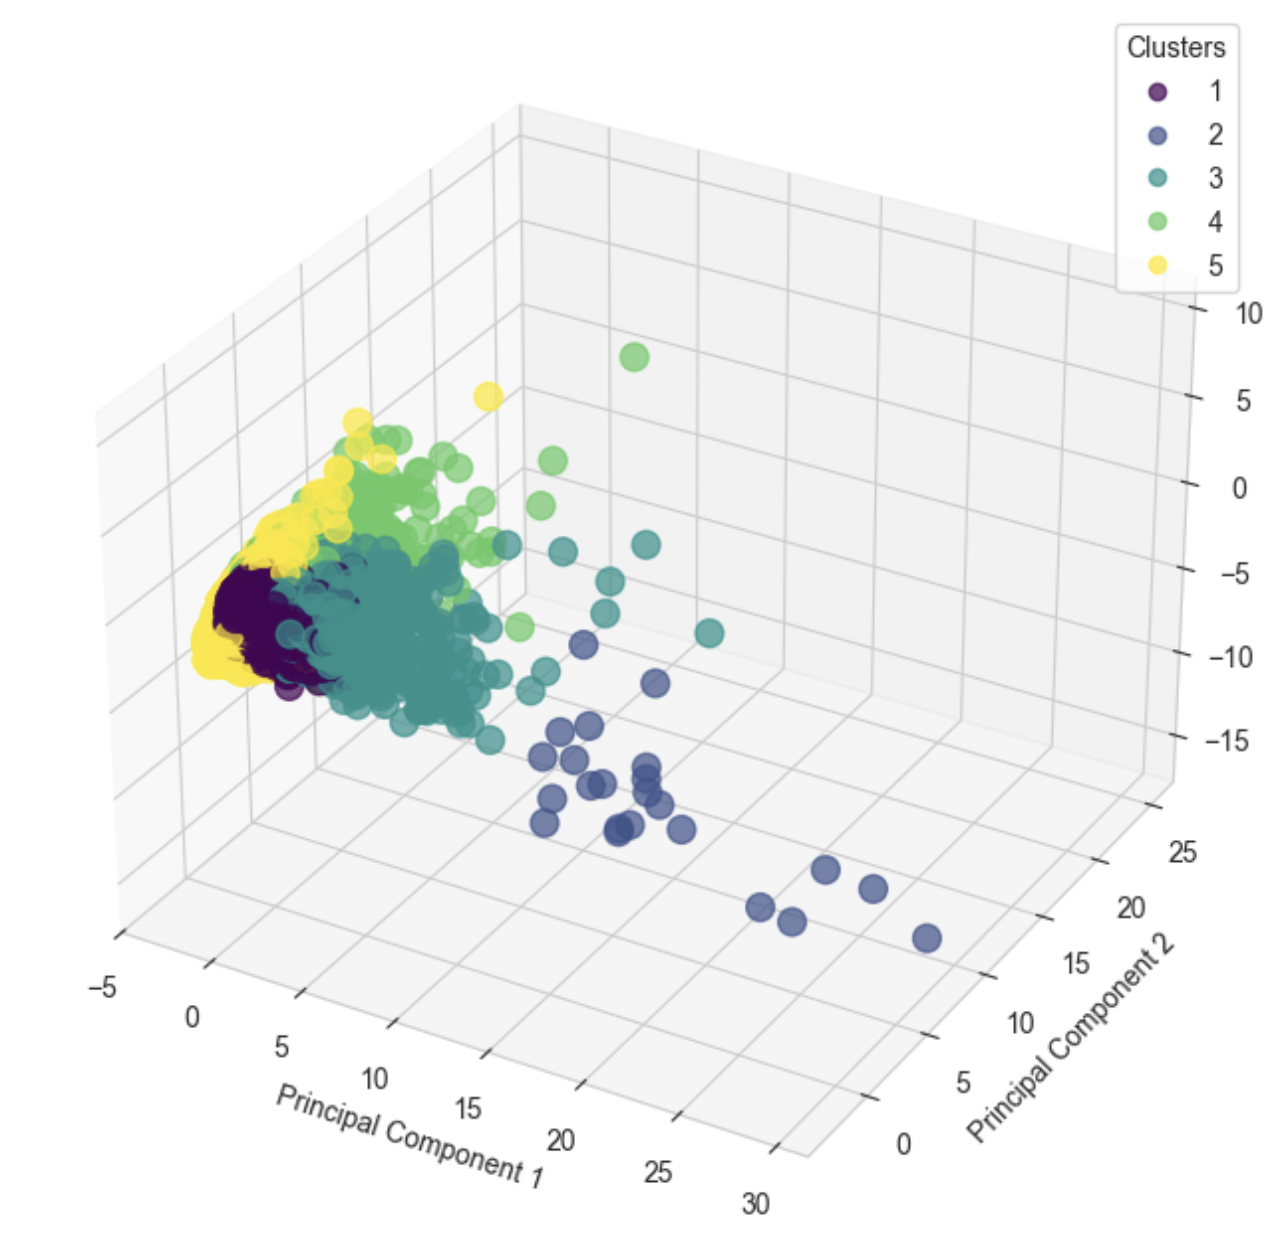
\includegraphics[width=\textwidth]{src/figs/3d_PCA_HC.png}
        \caption{3D PCA}
        \label{fig:3D_pca}
    \end{subfigure}
    \hfill
    \begin{subfigure}[b]{0.45\textwidth}
        \centering
        \raisebox{0.3cm}{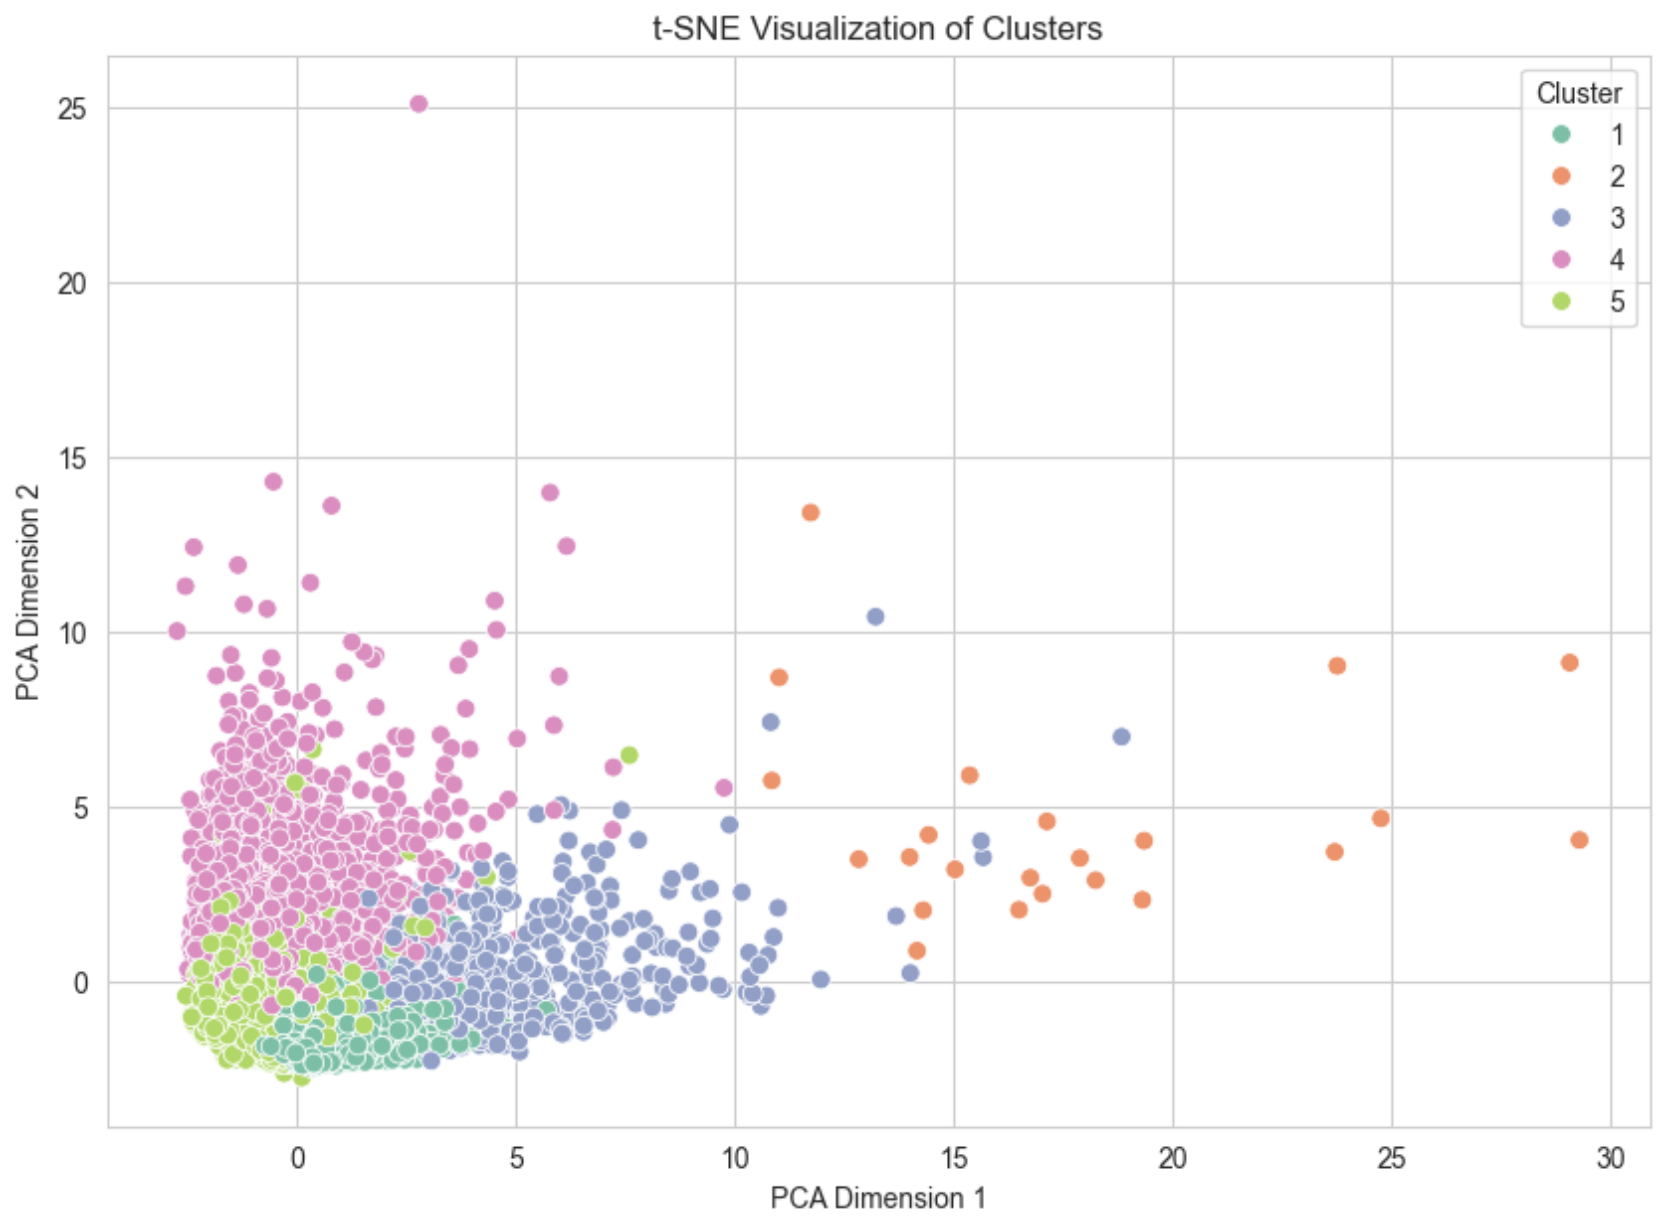
\includegraphics[width=\textwidth]{src/figs/2d_PCA_HC.png}} % Adjusts the image height
        \caption{2D PCA}
        \label{fig:PCA_2d}
    \end{subfigure}
    \caption{Clustering visualizations: 3D (left) and 2D (right).}
    \label{fig:comparison1}
\end{figure}

\begin{figure}[H]
    \centering
    \begin{subfigure}[b]{0.45\textwidth}
        \centering
        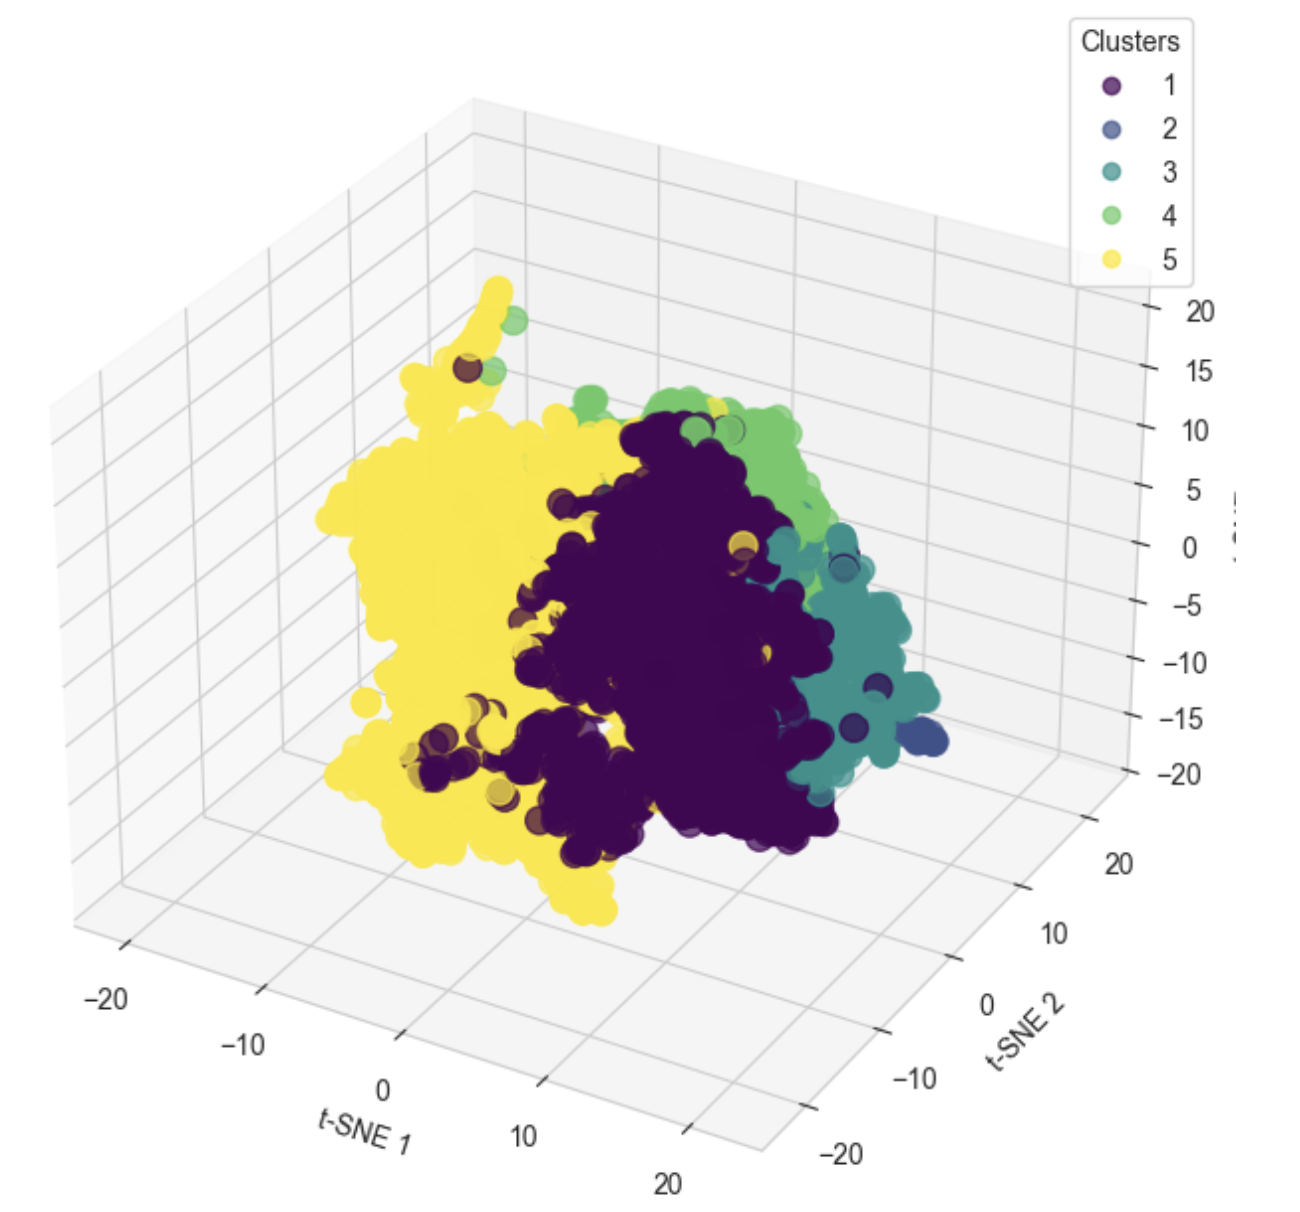
\includegraphics[width=\textwidth]{src/figs/3d_t-SNE.png}
        \caption{3D t-SNE}
        \label{fig:3D_tsne}
    \end{subfigure}
    \hfill
    \begin{subfigure}[b]{0.45\textwidth}
        \centering
        \raisebox{0.3cm}{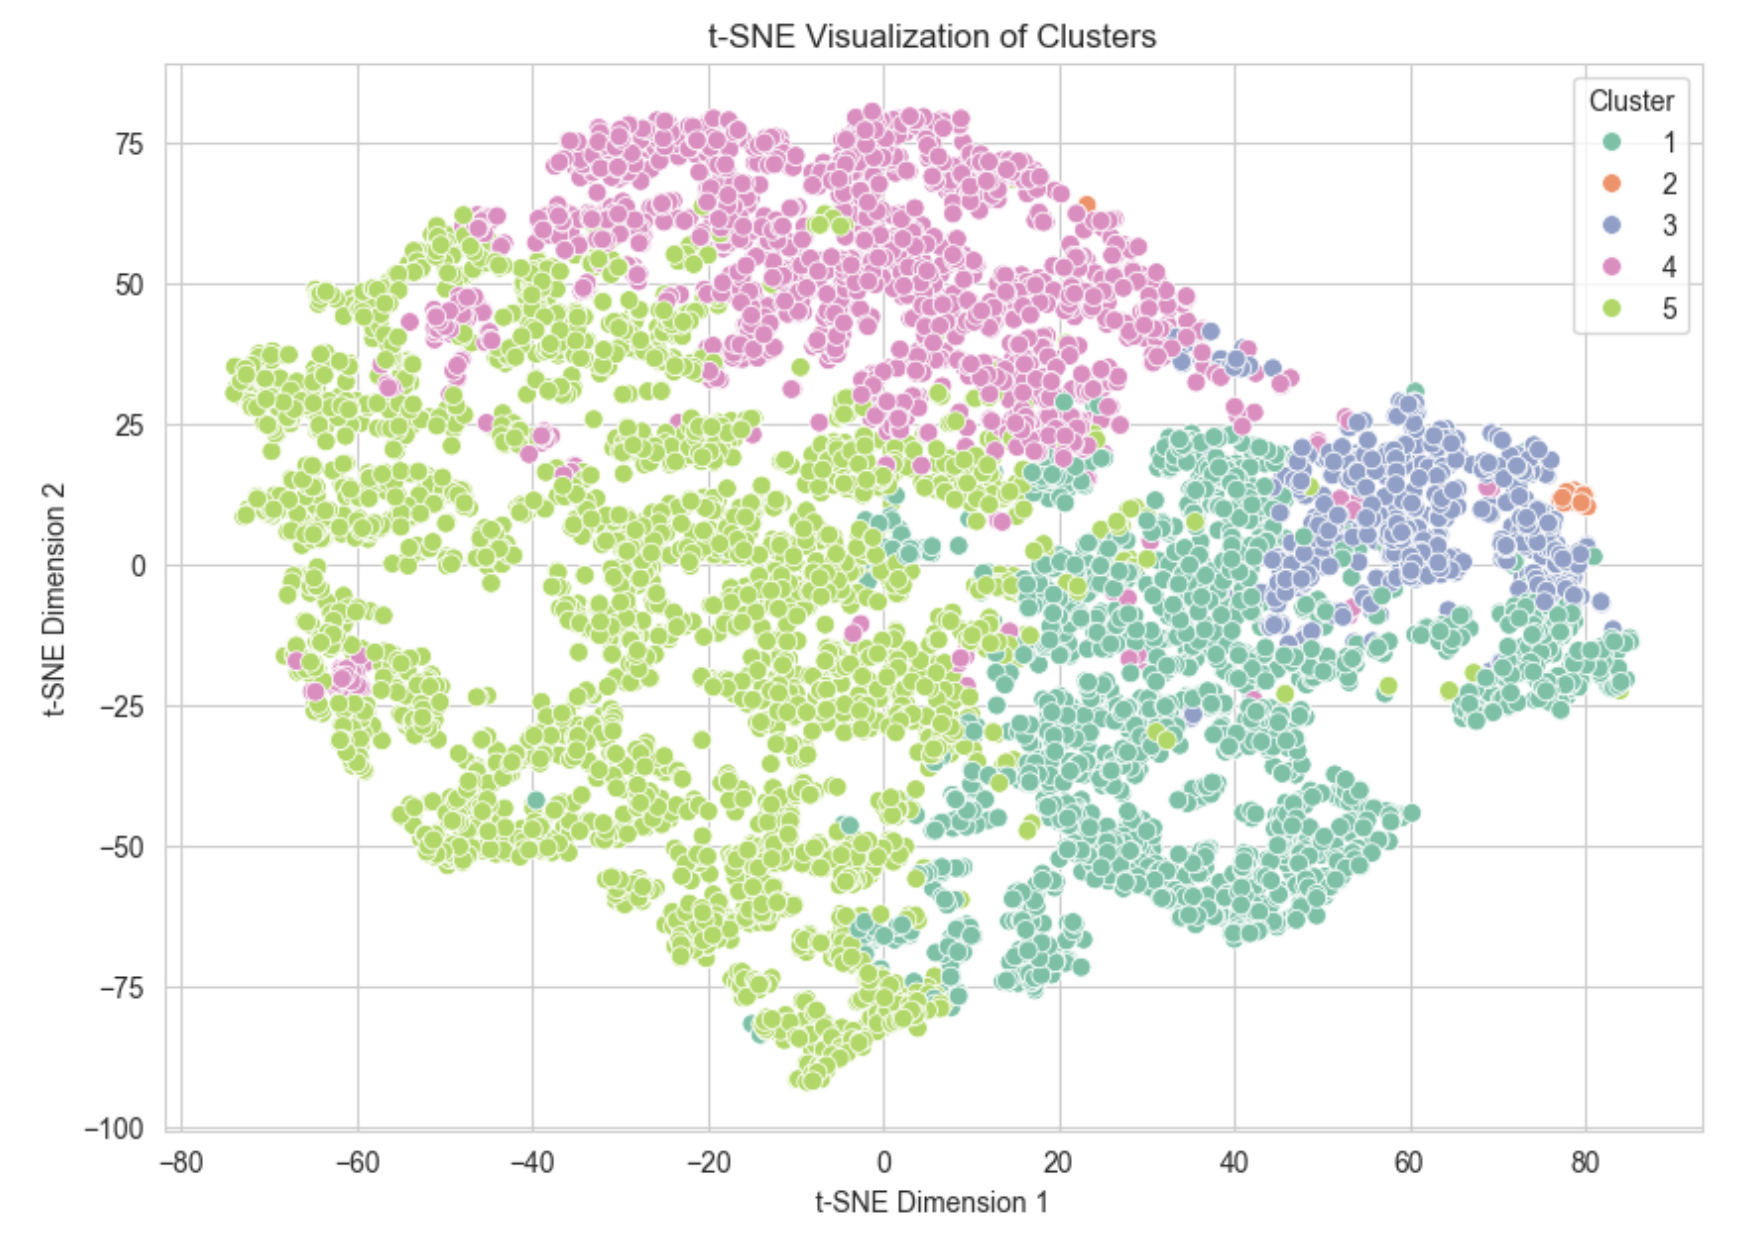
\includegraphics[width=\textwidth]{src/figs/2d_t-SNE.png}} % Adjusts the image height
        \caption{2D t-SNE}
        \label{fig:2D_tsne}
    \end{subfigure}
    \caption{Clustering visualizations: 3D (left) and 2D (right).}
    \label{fig:comparison2}
\end{figure}

\subsubsection{Cluster Descriptions}
Clarification on what the clusters contain and represent.
Values are represented by the mean of each cluster, except for the cluster size, which is calculated as the sum of all data points in the cluster.  

\vspace{0.3cm}
\par

\begin{center}


\noindent
\begin{minipage}[t]{0.48\textwidth}
\centering
\textbf{Cluster 1: Medium Activity, Low Spenders with Higher Full Payment Rate}
\vspace{0.2cm}
\resizebox{\textwidth}{!}{
\begin{tabular}{|l|c|c|}
\hline
\rowcolor{gray!50}
\textbf{Feature} & \textbf{Values} & \textbf{Interpretation} \\ \hline
Balance & 587.98 & Low \\ \hline
Purchases & 1203.26 & Low \\ \hline
One-Off Purchases & 542.97 & Moderate \\ \hline
Installments Purchases & 660.38 & Moderate \\ \hline
Cash Advance & 69.96 & Low \\ \hline
Credit Limit & 4157.06 & Moderate \\ \hline
Payments & 1269.62 & Moderate \\ \hline
Full Payment Percentage & 0.35 & Moderate \\ \hline
Cluster size & 2228.00 & Moderate \\ \hline
\end{tabular}}
\captionof{table}{Cluster 1 description.}
\end{minipage}
\hfill
\begin{minipage}[t]{0.48\textwidth}
\centering
\textbf{Cluster 2: High Spenders with Large Balances and High Full Payment Rate}
\vspace{0.2cm}
\resizebox{\textwidth}{!}{
\begin{tabular}{|l|c|c|}
\hline
\rowcolor{gray!50}
\textbf{Feature} & \textbf{Values} & \textbf{Interpretation} \\ \hline
Balance & 4812.38 & Very High \\ \hline
Purchases & 27505.34 & Very High \\ \hline
One-Off Purchases & 22417.45 & Very High \\ \hline
Installments Purchases & 5087.89 & Very High \\ \hline
Cash Advance & 1617.79 & High \\ \hline
Credit Limit & 16000.00 & Very High \\ \hline
Payments & 28138.98 & Very High \\ \hline
Full Payment Percentage & 0.53 & High \\ \hline
Cluster size & 23.00 & Very Low \\ \hline
\end{tabular}}
\captionof{table}{Cluster 2 description.}
\end{minipage}

\vspace{0.7cm}

\noindent
\begin{minipage}[t]{0.48\textwidth}
\centering
\textbf{Cluster 3: Moderate Credit Usage with Low Full Payment Rate}
\vspace{0.2cm}
\resizebox{\textwidth}{!}{
\begin{tabular}{|l|c|c|}
\hline
\rowcolor{gray!50}
\textbf{Feature} & \textbf{Values} & \textbf{Interpretation} \\ \hline
Balance & 3093.29 & High \\ \hline
Purchases & 5059.38 & Moderate \\ \hline
One-Off Purchases & 3176.73 & Moderate \\ \hline
Installments Purchases & 1883.64 & Moderate \\ \hline
Cash Advance & 427.99 & Moderate \\ \hline
Credit Limit & 8084.07 & High \\ \hline
Payments & 4411.09 & Moderate \\ \hline
Full Payment Percentage & 0.18 & Low \\ \hline
Cluster size & 609.00 & Low \\ \hline
\end{tabular}}
\captionof{table}{Cluster 3 description.}
\end{minipage}
\hfill
\begin{minipage}[t]{0.48\textwidth}
\centering
\textbf{Cluster 4: Customers with Low Purchases, High Cash Advances, and Low Full Payment}
\vspace{0.2cm}
\resizebox{\textwidth}{!}{
\begin{tabular}{|l|c|c|}
\hline
\rowcolor{gray!50}
\textbf{Feature} & \textbf{Values} & \textbf{Interpretation} \\ \hline
Balance & 3753.04 & High \\ \hline
Purchases & 536.14 & Low \\ \hline
One-Off Purchases & 311.82 & Low \\ \hline
Installments Purchases & 224.39 & Low \\ \hline
Cash Advance & 3412.73 & Very High \\ \hline
Credit Limit & 6304.57 & High \\ \hline
Payments & 2908.71 & Low \\ \hline
Full Payment Percentage & 0.04 & Low \\ \hline
Cluster size & 1796.00 & Moderate \\ \hline
\end{tabular}}
\captionof{table}{Cluster 4 description.}
\end{minipage}

\vspace{0.7cm}


\noindent
\begin{minipage}[t]{0.48\textwidth}
\centering
\textbf{Cluster 5: Low Usage of Credit with Minimal Purchases or Payments}
\vspace{0.2cm}
\resizebox{\textwidth}{!}{
\begin{tabular}{|l|c|c|}
\hline
\rowcolor{gray!50}
\textbf{Feature} & \textbf{Values} & \textbf{Interpretation} \\ \hline
Balance & 950.55 & Low \\ \hline
Purchases & 376.41 & Low \\ \hline
One-Off Purchases & 252.25 & Low \\ \hline
Installments Purchases & 124.60 & Low \\ \hline
Cash Advance & 503.19 & Low \\ \hline
Credit Limit & 3310.72 & Low \\ \hline
Payments & 1011.16 & Low \\ \hline
Full Payment Percentage & 0.10 & Low \\ \hline
Cluster size & 3980.00 & High \\ \hline
\end{tabular}}
\captionof{table}{Cluster 5 description.}
\end{minipage}

\end{center}


\subsection{DBSCAN}

\subsubsection{Evaluation}

\begin{figure}[H]
    \centering
    \begin{tabular}{|l|c|}
        \hline
        \rowcolor{gray!50}
        & Value \\ \hline
        \textbf{Silhouette Score} & $-0.328$ \\ \hline
        \textbf{Dunn Index} & $0.001$ \\ \hline
    \end{tabular}
    \caption{Evaluation metrics for DBSCAN}\label{fig:DBSCAN_evaluation}
\end{figure}

\subsubsection{Visualization of the clusters:}

The clusters we get from DBSCAN are visualized in 3D using PCA and t-SNE. First we visualize the clusters including the $-1$ cluster, which represents the outliers. Then we visualize the clusters without the $-1$ cluster, to get a better view of the clusters that DBSCAN finds.

\begin{figure}[H]
    \hspace*{\fill}
    \centering
    \begin{subfigure}[b]{0.45\textwidth}
        \centering
        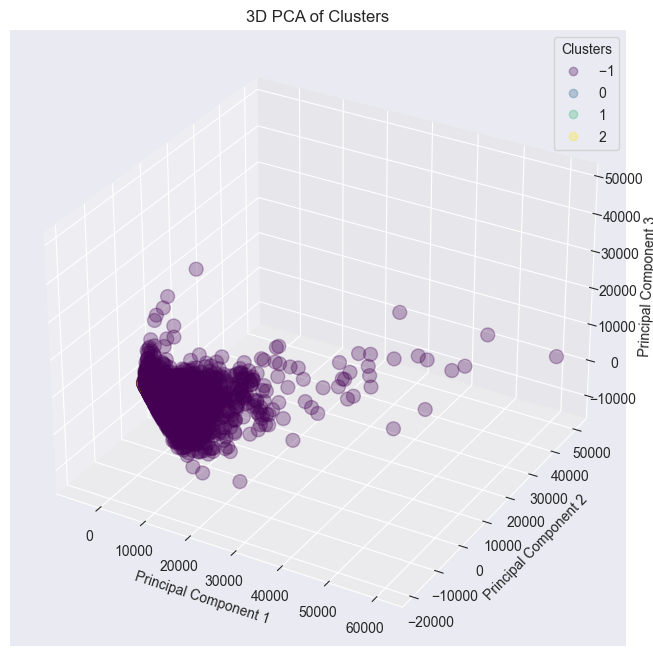
\includegraphics[width=1.0\textwidth]{src/figs/3d_PCA_DBSCAN_with.png} 
        \caption{3D PCA with $-1$ cluster}\label{fig:DBSCAN_PCA_with}
    \end{subfigure}
    \hfill
    \begin{subfigure}[b]{0.45\textwidth}
        \centering
        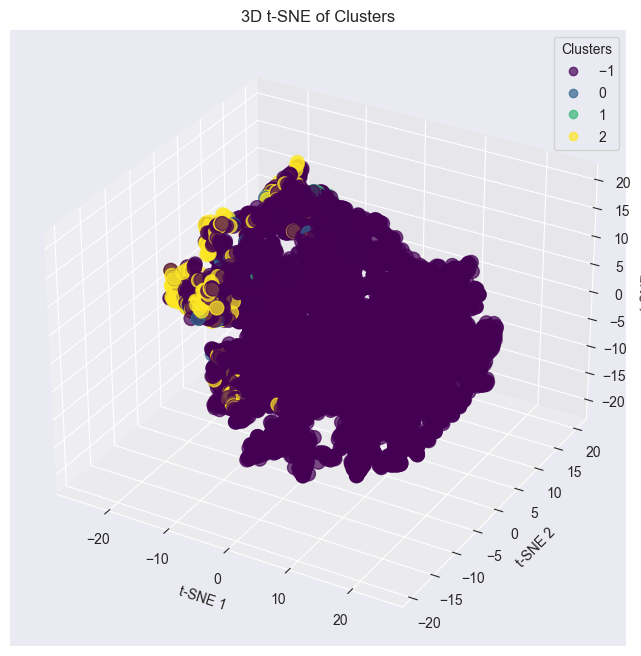
\includegraphics[width=1.0\textwidth]{src/figs/3d_t-SNE_DBSCAN_with.png} 
        \caption{3D t-SNE with $-1$ cluster}\label{fig:DBSCAN_tsne_with}
    \end{subfigure}
    \caption{Visualization of DBSCAN clusters with $-1$ cluster data included}\label{fig:with_outliers}
    \hspace*{\fill}
\end{figure}

\begin{figure}[H]
    \hspace*{\fill}
    \centering
    \begin{subfigure}[b]{0.45\textwidth}
        \centering
        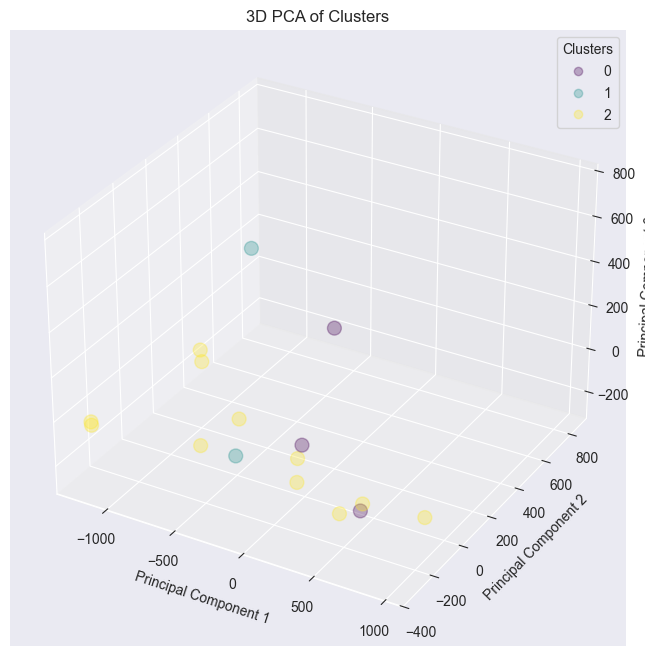
\includegraphics[width=1.0\textwidth]{src/figs/3d_PCA_DBSCAN_without.png} 
        \caption{3D PCA without $-1$ cluster}\label{fig:DBSCAN_PCA_without}
    \end{subfigure}
    \hfill
    \begin{subfigure}[b]{0.45\textwidth}
        \centering
        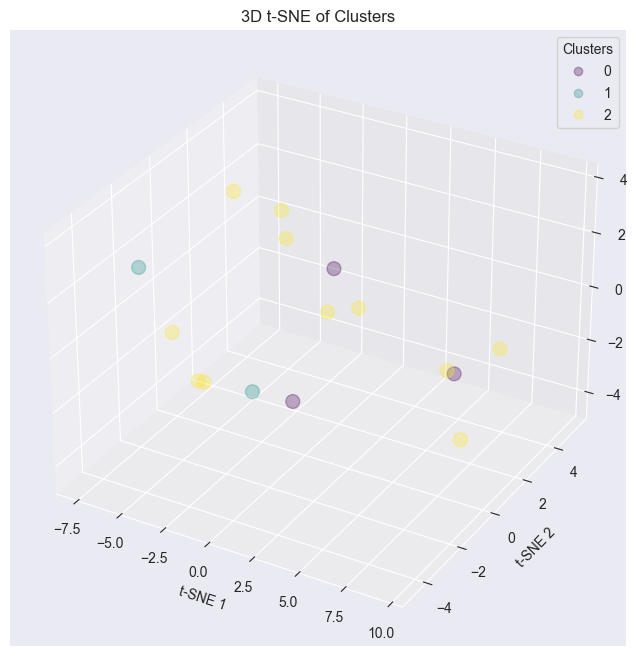
\includegraphics[width=1.0\textwidth]{src/figs/3d_t-SNE_DBSCAN_without.png} 
        \caption{3D t-SNE without $-1$ cluster}\label{fig:DBSCAN_tsne_without}
    \end{subfigure}
    \caption{Visualization of DBSCAN clusters with $-1$ cluster data excluded}\label{fig:without_outliers}
    \hspace*{\fill}
\end{figure}
\section{Discussion}

\subsection{Ethical consideration}

Our implementation of a machine learning model to classify bottles in a factory brings a few important ethical considerations. 
While the technology offers great improvements in quality control and efficiency, it also presents challenges that need to be discussed and thought about.

First of is data security and privacy. 
The system processes large amounts of production data that could be valuable to competitors. 
Factories that uses our implementation is therefore recommended to implement a robust cybersecurity system to protect against industrial espionage and unauthorized access. 
This includes secure data storage, encrypted communications, and strict access controls for system modifications.

Additionally, our implementation leads to workforce changes. While some traditional quality control positions may be displaced, new roles emerge in system maintenance, monitoring, and data analysis. 
This transformation requires human resources, they should present retraining programs and use clear communication with affected employees.
To ensure employees gets the right and fair treatment.

Finally, accountability and responsibility of our implementation present another critical consideration. 
If defective products reach customers, clear frameworks must be establish whether responsibility lies with the system developers, factory management, or quality control staff. 
This requires transparent documentation of the system's decision-making process and regular reviews of its performance.

In conclusion, ethical implications of implementing this technology extend beyond the factory product line.
While automation can improve product quality and reduce waste, organizations must balance these benefits against their social responsibilities. 
This includes maintaining employment opportunities while adapting to technological advancement, ensuring transparent communication with stakeholders, and maintaining human oversight in critical decision-making processes.

\subsection{Limitations}

• Inte riktig data
• Fake noise, riktigt noise skulle vara damm och smuts på linsen tex.
\section{Conclusion}

Our paper demonstrates the effectiveness of an autoencoder-based anomaly detection system combined with a CNN for classifying bottle defects, while still using a small dataset.
The anomaly detection procedure accurately identifies anomalies with minimal errors, and the CNN successfully classifies the defects. 
However, consider the limitations such as reliance on synthetic data, overrepresentation of a certain class, and the introduction of synthetic noise may affect the performance in the real world.
While the model performs well in a controlled setting, its generalizability to actual factory conditions remains unknown.

Future improvements include testing alternative architectures, enhancing data augmentation techniques, and deploying the model in a real production environment to collect authentic defect data. 
Ethical considerations such as data security, workforce impact, and accountability must also be addressed when implementing such systems in industry. 
Overall, this paper highlights the potential of deep learning for automated defect detection, but further validation by applications in the real world is necessary to ensure reliability and robustness.

\end{document}
